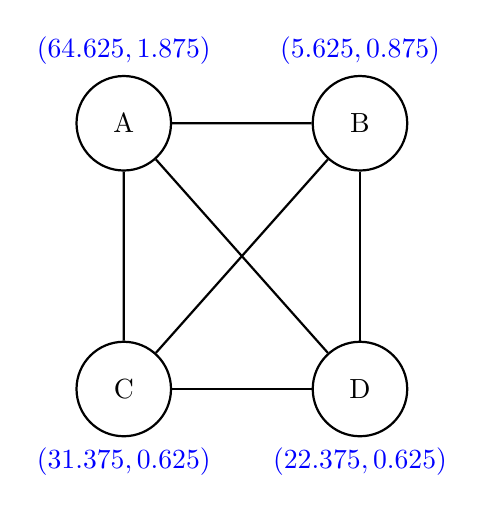
\begin{tikzpicture}[scale=0.75, thick, main node/.style={circle, draw, minimum size=1.2cm}]

    % First graph
    \node[main node] (A1) at (-1,4.5) {A};
    \node[main node] (B1) at (3,4.5) {B};
    \node[main node] (C1) at (-1,0) {C};
    \node[main node] (D1) at (3,0) {D};
    
    \node[above, color=blue] at (A1.north) {$(64.625,1.875)$};
    \node[above, color=blue] at (B1.north) {$(5.625, 0.875)$};
    \node[below, color=blue] at (C1.south) {$(31.375, 0.625)$};
    \node[below, color=blue] at (D1.south) {$(22.375, 0.625)$};
    
    \draw (A1) -- (B1);
    \draw (A1) -- (C1);
    \draw (A1) -- (D1);
    \draw (B1) -- (C1);
    \draw (B1) -- (D1);
    \draw (C1) -- (D1);

\end{tikzpicture}